\documentclass[12pt]{article}
\usepackage{geometry}
\geometry{a4paper}
\usepackage[round]{natbib}
\usepackage{graphicx}
\usepackage[T1]{fontenc}
\usepackage[utf8]{inputenc}
\usepackage{textcomp}
\usepackage{gensymb}
\usepackage{hyperref}
\usepackage{amsmath}
\usepackage{amssymb}
\usepackage{authblk}
\usepackage[running]{lineno}
\usepackage{setspace}
\usepackage{rotating}

\setlength{\parindent}{0pt}


\usepackage{fancyhdr}
 
\pagestyle{fancy}
\fancyhf{}
\rhead{Tad Dallas (Biol 4253)}
\lhead{ Metapopulations and island biogeography}

\doublespacing


\begin{document}





\subsection*{Reading:}


Gotelli, Nicholas J. A primer of ecology. Sunderland, MA: Sinauer Associates, 2001. Chapter 4. \\

\bigskip

Yu, Angela D.; Lei, Simon A. 2001. Equilibrium theory of island biogeography: A review. In: McArthur, E. Durant; Fairbanks, Daniel J., comps. Shrubland ecosystem genetics and biodiversity: proceedings; 2000 June 13-15; Provo, UT. Proc. RMRS-P-21. Ogden, UT: U.S. Department of Agriculture, Forest Service, Rocky Mountain Research Station. p. 163-171. \url{https://www.fs.fed.us/rm/pubs/rmrs_p021/rmrs_p021_163_171.pdf}















\begin{center}
\noindent\hrulefill 
\end{center}





\clearpage

\subsection*{How does landscape structure influence population processes?}

Alright. So we've studied species population processes, their abiotic tolerances (the niche), and community composition and assembly processes. But we haven't dealt directly with the role of dispersal and spatial habitat distribution on resulting species dynamics. This week, we'll remedy this, by exploring two bodies of theory related to interconnected populations and communities at the landscape level. 





\bigskip


\subsection*{Huffaker's mites and the importance of spatial processes}

In the late 1950's, Huffaker started an experiment with pretty similar intent to Gause's experiment using protists, which served as the basis for the idea of competitive exclusion. Here, Huffaker wanted to explore how spatial processes influenced predator-prey interactions. The system he set up was a series of oranges (resource) connected by little corridors to allow dispersal of a mite consumer (of the oranges). On top of this, he added a predator of the mites (also a mite). He found a number of cool things, which we'll break down point by point.


\begin{itemize}

  \item In no-predator experiments, the spatial distribution of patches allowed for more stable consumer population dynamics. Without spatial structure (oranges clumped nearby one another), consumer populations grew large, depleted resource, and then crashed.

  \item Prey refugia super important to maintaining coexistence. Huffaker went through pains to make a situation which would potentially allow coexistence. Dispersal corridors were made more difficult for predators to traverse, orange balls replaced oranges to provide spatial variation in food resource, parts of each orange were sealed with parafin wax to control resource amount, etc. 

  \item Predator-prey oscillations are possible to observe in experiments -- or rather, oscillation, as a maximum of 1 clear oscillation before extinction was observed for any treatment -- but are influenced by spatial heterogeneity of resource and dispersal processes.

\end{itemize}


And this was before we had really coined the term "metapopulation" and thought about spatial processes in this way. 













\bigskip

\subsection*{Scaling populations to landscapes}

Populations of a single species may be distributed across a landscape of suitable habitat patches within a larger landscape of unsuitable landscape. Consider an aquatic plant species across a mostly terrestrial landscape dotted with lakes. The species can only exist in the lake habitats, but these lakes can be connected through dispersal processes. This set of lake habitats connected by dispersal comprises a \textit{metapopulation}. 

Metapopulations are considered to be in a relatively constant state of flux, as \textit{local extinctions} -- single populations that go to extinction -- of species in habitat patches are buffered by re-colonization by dispersal from neighboring patches. In this way, dispersal can be beneficial or detrimental to metapopulation persistence. 


Under high dispersal, patches become homogeneous and population dynamics tend to become synchronous. This \textit{synchrony} is destabilizing, in that periods of low population sizes will be experienced by all patches, increasing the likelihood of stochastic extinction of the entire metapopulation. On the other hand, too little dispersal will result in spatial clustering of a species, as the species will be confined to the set of patches that can be successfully reached and colonized and similarly potentially increasing extinction risk.









\bigskip

\subsection*{The benefits of a metapopulation}

Consider a population existing on a single patch with some probability of extinction ($P_e$) of 0.2. Extinction risk at any timepoint is independent of the previous timepoint (a big assumption, but bear with me). The probability of population persistence for a 5 year period is then (1- $P_e$)$^{5}$ or 0.328, which corresponds to a probability of extinction of 0.672. If we were to divide this single patch into two patches, and make the assumption that extinction risk is the same (not a terribly big assumption, but we'll address this later). Regional extinction (both patches going extinct) would be equal to $P_{e}^{2}$, so the probability of regional extinction sometime within a period of 5 years would be  1 - probability of persistence = 1 - $\left((1 - P_e^{2})^{5}\right)$. This would suggest that the persistence probability now is 0.815, and the risk of extinction has therefore dropped to 0.185. 

















\bigskip


\subsection*{How do metapopulations work?}

To understand metapopulations, we'll start with a foundational metapopulation model; the Levins' model. Levins created a simple model focused solely on patch occupancy (i.e., is the species present or absent) as a way to mathematically assess the proportion of occupied patches by a species given minimal demographic information. In this case, local habitat patches are either occupied or unoccupied, and both patch number and the spatial orientation of patches are undescribed. Dispersal among habitat patches can rescue patches from extinction, or allow for the recolonization of extinct patches. All patches are treated as equal, so that any patch is suitable for a species, and (as a simplifying assumption) all habitat patches can be reached from all other patches. This simplified representation treats space as implicit, and patch quality and size as constant; rather than an explicit population size, patch occupancy is just a 0 or 1 state.


\begin{equation}
\frac{dN}{dt} = cN(1-N) - eN
\end{equation}

where the change in the number of occupied sites ($N$) by a species is a function of colonization rate $c$ and extinction rate $e$. 


This should look somewhat familiar, but if it doesn't, no worries. It can be expressed using similar things from the logistic model, which we went over when discussing population dynamics and Lotka-Volterra competition. But here, the carrying capacity (which was the number of individuals a site could support in the population dynamics lecture) is now the fraction of patches that will be occupied by a species at equilibrium. 

The equilibrium fraction of patches that should be occupied via colonization and extinction rates is 

\begin{equation}
K = 1 - \frac{e}{c}
\end{equation}

Further, this model can be used to generate a threshold condition for metapopulation persistence, which relates to the balance between colonization and extinction rates, and is analagous to population growth rate in the logistic model. That is, a metapoulation will persist if 


\begin{equation}
  \frac{e}{c} < 1 
\end{equation}


That is, when extinction rate becomes larger than colonization, the metapopulation will not persist. This shows that even a metapopulation in equilibrium is still in a constant state of patch-level flux. In real applications, this implies that just because a patch of habitat is empty, that may not imply it is uninhabitable; and similarly, just because a population goes extinct, it may not be indicative of broader declines or instability.


This is admittedly a simple representation of a metapopulation, as it assumes that all habitat patches are equivalent (colonization and extinction rates are constant across patches), there is no spatially-explicit structure to the distribution of patches, and the only thing we track is occupancy (so population dynamics within a single patch are not considered). 




Assumptions of the Levins model:
\begin{itemize}
  \item patches are all the same
  \item no spatial structure 
  \item constant $e$ and $c$, 

\end{itemize} 


However, despite this simplicity, the Levins model can yield important insights into spatial population dynamics. For instance, the mean time to extinction of any given population/patch is the inverse of the rate (i.e., $T_E = \frac{1}{e}$). The simplicity of the Levins model has resulted in a sizable body of literature surrounding and extending the model. For instance, in the original Levins' model all patches are equidistant from one another, identical in quality, and can only be in one of two potential states (occupied or unoccupied), but each of these conditions is frequently adjusted in derivative stochastic patch occupancy models (SPOMs). Researchers have shown that despite the simplicity, Levins-type dynamics can emerge from more complicated stochastic metapopulation models, and extensions of the Levins model continue to provide insight into the influence of habitat patch size and topography (i.e., spatial orientation of habitat patches) on metapopulation persistence.











\bigskip

\subsection*{Types of metapopulations}

Metapopulation "type" can be divided along two axes, which describe the dispersal connections between habitat patches and the relative size of habitat patches. That is, we can imagine a 2-dimensional space, where one axis corresponds to connectivity (how well are patches connected by dispersal?) and the other axis corresponds to variance in patch size (what is the distribution of patch sizes in the metapopulation?) 


\begin{figure}

  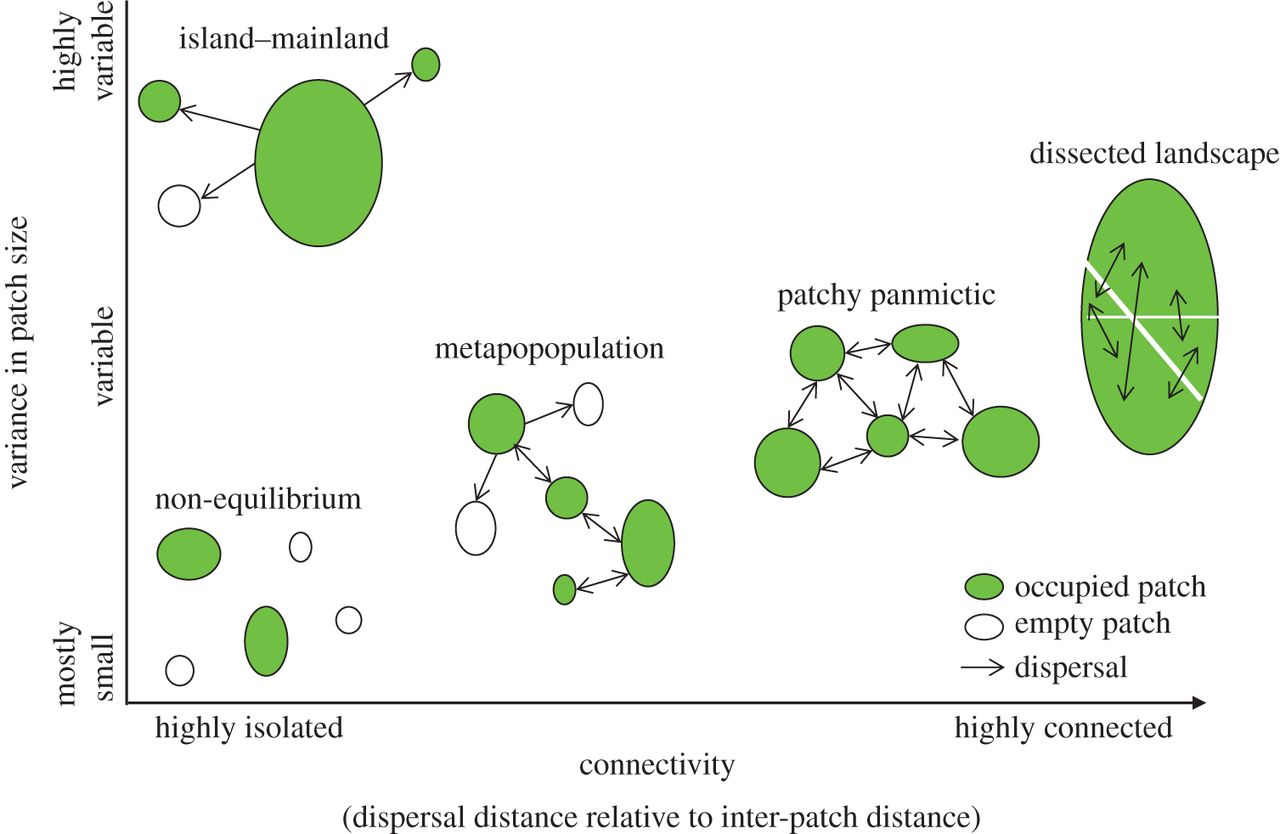
\includegraphics[width=0.75\textwidth]{figs/MP1.jpg}
  \caption{Taken from https://naes.unr.edu/shoemaker/teaching/NRES-470/LECTURE13.html}

\end{figure}






\bigskip

\subsection*{Mainland-Island model}

Colonization comes from a single source, and isn't dependent on the fraction of occupied patches. This basically assumes the idea of "propagule rain", that a constant supply of immigrants are provided and patches become colonized from this mainland source.

\begin{equation}
\frac{dN}{dt} = c(1-N) - eN
\end{equation}


This changes our equilibrium fraction of occupied patches though. Making this assumption shifts the metapopulation $K$ to 

\begin{equation}
K = \frac{c}{c+e}
\end{equation}


Note here the effects of the propagule rain. Across a large range of extinction rates ($e$), $K$ still may be relative unaffected. That is, colonization processes become far more important here, as the fraction of occupied patches at equilibrium is now basically the fraction of colonization relative to extinction. This also brings up the existence of \textit{sources} and \textit{sinks}. The mainland is assumed to be a \textit{source} here, defined as those patches with positive growth rates even in the presence of emigration (these patches are creating a bunch of individuals and then those individuals are dispersing). \textit{Sink} populations are those that persist, but have a negative population growth rate, such that they are only maintained via immigration of individuals from other patches. 






\bigskip

\subsection*{Patchy Population}

Local populations exist, but patches are so well-connected via dispersal that interbreeding is common and individuals may occupy any patch in the system. These systems tend to have high patch occupancy, and are \textit{not} considered metapopulations by most scientists. 









\bigskip

\subsection*{Non-equilibrium Populations}

Local populations exist, but patches that go extinct are rarely re-colonized (as a function of low dispersal). Each population is pretty independent, and their demographics are not linked (via immigration/emigration). These systems are pretty much destined for extinction (as extinction rates often exceed colonization rates), and are \textit{not} considered metapopulations by most scientists. 







































\bigskip

\subsection*{The rescue effect}

Above, we treated the probability of extinction as independent from the fraction of occupied patches. However, what if local patch-level extinction probability ($e$) was a function of the fraction of occupied patches($N$)? Dispersal individuals from occupied sites serve not only to (re)colonize habitat patches, but also to provide individuals to other already established populations. Thus, a population that may have gone extinct due to small population sizes or demographic/environmental stochasticity now will not go extinct due to this extra boost from nearby populations. This boost is the \textit{rescue effect}, and was incorporated into the Levins model by Hanski in 1982. 



Let's consider the probability of extinction to depend inversely on the fraction of occupied patches (i.e., more patches occupied means fewer extinctions are going to occur). We now consider $e$ to be similar to the colonization rate, which depends on the fraction of occupied patches and the availability of unoccupied patches. 


This changes the classic Levins model

\begin{equation}
\frac{dN}{dt} = cN(1-N) - eN
\end{equation}

by making $e$ a function of $N$, and results in the following

\begin{equation}
\frac{dN}{dt} = cN(1-N) - eN(1-N)
\end{equation}

which doesn't change the persistence conditions for the metapopulation as described above.















\bigskip

\subsection*{Removal of patches}

One interesting thing about metapopulations is that empty patches serve a role in metapopulation persistence. This has clear implications to conservation, as even the destruction of habitat where no organisms presently exist could affect the extinction probability of many species.


\begin{equation}
\frac{dN}{dt} = cN(1-N-D) - eN
\end{equation}

where $D$ is the proportion of patches removed from the system. This makes the equilibrium now

\begin{equation}
K = 1 - \frac{e}{c} - D
\end{equation}




















\bigskip

\subsection*{Incorporating the influence of patch area and distance between patches}

An extension of the Levins model provides a bridge between metapopulations and island biogeography theory (which will discuss further next). This simple extension considers a set of spatially explicit patches of variable size, where a distance matrix $D$ describes the distance between all patches in the metapopulation. The model borrows elements of MacArthur and Wilson's \textit{Theory of Island Biogeography}, such that distance between patches ($D_{ij}$) and patch area ($A_{i}$) influence extinction and colonization processes, where the patch extinction rate scales with patch area ($e_{i} = e / A_{i}$), and colonization ($c_{i}$) becomes a property of distance ($D_{ij}$), patch area ($A_{i}$), and dispersal rate ($\alpha$) where  


\begin{equation}
c_{i} = \sum_{j \ne i}e^{-\alpha D_{ij}} A_{j}p_{j}(t)
\end{equation}


\noindent This suggests that the mean time to extinction of a habitat patch ($1 / e_{i}$) is determined by the area of the patch. 















































































\clearpage
\subsection*{What is the theory of island biogeography?}

As discussed above with respect to patch occupancy in metapopulations, the \textit{theory of island biogeography} attempts to explain the colonization and extinction of species (and subsequently the species richness of islands) as a function of island area and distance from the mainland. These two things influence the number of species that can colonize and persist on a given island, as distance from a mainland source is proportional to species dispersal and colonization probability and island area controls the population size attainable by a given species, and thus influences extinction rate. That is, the theory is based on the relationship between distance from the mainland (colonization rate) and island area (extinction rate) in determining the number of species that an island contains. 



This is fundamentally related to a metapopulation, as the structure of the landscape is the same. That is, a metapopulation consists of habitat patches connected by dispersal but within an inhospitable landscape. The theory of island biogeography assumes the same, originally developed to explain the number of species on isolated islands. 



This assumes that all islands are reachable by every species in the community with a non-zero probability, and is spatially-implicit (i.e., the actual locations of habitat patches are not considered). 
















\bigskip

\subsection*{Species-area relationships}

One clear extension, and honestly the original purpose of island biogeography theory, is the study of species-area relationships. The idea here is that increasing geographic area results in a greater number of unique species able to occupy the patch. 


Species-area relationships exist in two different forms, depending on how the data are structured. The most related to island biogeography theory is the "island" species-area relationship, where a set of discontiguous habitats are studied, and the area of each patch is related to species richness in that patch. The second -- called the "mainland" species-area relationship -- considers a contiguous habitat where patches are nested within another.




\begin{equation}
S = cA^{z}
\end{equation}



where $S$ is the number of species, $A$ is patch area, $z$ describes the shape of the relationships, and $c$ is a constant. $c$ actually describes the number of species we would expect to find in one unit of sampling area (whatever the unit is in the study).  



The utility of this simple formula is that it suggests that the number of species is a simple function of area, which can help aid in the design of research (how big of a sampling area is required to truly characterize a community?), and to estimate species richness for unobserved sites of known area (is it possible to estimate the number of species on an island we've never been to?). 


One interesting point is that both the theory of island biogeography and the species-area relationship make the assumption that species colonization and extinction rates are only a function of island area and distance to mainland. That is, species do not fundamentally differ in their dispersal rates, or only do so in a proportional way to one another as a function of island area and isolation (distance to mainland). 




























\iffalse

\bigskip

\subsection*{Hanski's incidence function model}

Spatially-explicit model. 

\[J_i = \frac{c_{i}}{c_{i} + e_{i} - (e_{i}c_{i})} \]

\fi


\end{document}

